\documentclass[12pt]{article}
\usepackage[utf8]{inputenc}

\usepackage{lmodern}

\usepackage{enumitem}
\usepackage[margin=2cm]{geometry}

\usepackage{amsmath, amsfonts, amssymb}
\usepackage{graphicx}
%\usepackage{subfigure}
\usepackage{tikz}
\usepackage{pgfplots}
\usepackage{multicol}

\usepackage{comment}
\usepackage{url}
\usepackage{calc}
\usepackage{subcaption}
\usepackage[indent=0pt]{parskip}
\usepackage{animate}

\usepackage{array}
\usepackage{blkarray,booktabs, bigstrut}
\usepackage{bigints}

\pgfplotsset{compat=1.16}

% MATH commands
\newcommand{\ga}{\left\langle}
\newcommand{\da}{\right\rangle}
\newcommand{\oa}{\left\lbrace}
\newcommand{\fa}{\right\rbrace}
\newcommand{\oc}{\left[}
\newcommand{\fc}{\right]}
\newcommand{\op}{\left(}
\newcommand{\fp}{\right)}

\newcommand{\bi}{\mathbf{i}}
\newcommand{\bj}{\mathbf{j}}
\newcommand{\bk}{\mathbf{k}}
\newcommand{\bF}{\mathbf{F}}

\newcommand{\mR}{\mathbb{R}}

\newcommand{\ra}{\rightarrow}
\newcommand{\Ra}{\Rightarrow}

\newcommand{\sech}{\mathrm{sech}\,}
\newcommand{\csch}{\mathrm{csch}\,}
\newcommand{\curl}{\mathrm{curl}\,}
\newcommand{\dive}{\mathrm{div}\,}

\newcommand{\ve}{\varepsilon}
\newcommand{\spc}{\vspace*{0.5cm}}

\DeclareMathOperator{\Ran}{Ran}
\DeclareMathOperator{\Dom}{Dom}

\newcommand{\exo}[1]{\noindent\textcolor{red}{\fbox{\textbf{Problem {#1}}}\hrulefill}\\}
\newcommand{\qu}[4]{\noindent\textcolor{#4}{\fbox{\textbf{Section {#1} | Problem {#2}}} \hrulefill{{\fbox{\textbf{{#3} Points}}}}\\}}

\newcommand{\semester}{Spring 2023}

\newcommand{\CVup}{%

\begin{tikzpicture}
\draw[black, <->, >=latex] (-0.33, 0.5) .. controls (-0.125, 0) and (0.125, 0) .. (0.33, 0.5);
\end{tikzpicture}}

\newcommand{\CVupInc}{%
\begin{tikzpicture}
\draw[black, ->, >=latex] (0,0) .. controls (0.2, 0) and (0.4, 0.2) .. (0.5, 0.5);
\end{tikzpicture}}

\newcommand{\CVupDec}{%
\begin{tikzpicture}[rotate=270]
\draw[black, ->, >=latex] (0,0) .. controls (0.2, 0) and (0.4, 0.2) .. (0.5, 0.5);
\end{tikzpicture}}

\newcommand{\CVdown}{%
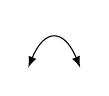
\begin{tikzpicture}
\draw[black, <->, >=latex] (-0.33, -0.5) .. controls (-0.125, 0) and (0.125, 0) .. (0.33, -0.5);
\end{tikzpicture}}

\newcommand{\CVdownInc}{%
\begin{tikzpicture}
\draw[black, ->, >=latex] (-0.5, -0.5) .. controls (-0.5, -0.3) and (-0.5, -0.1) .. (0,0);
\end{tikzpicture}}

\newcommand{\CVdownDec}{%
\begin{tikzpicture}[rotate=-90]
\draw[black, ->, >=latex] (-0.5, -0.5) .. controls (-0.5, -0.3) and (-0.5, -0.1) .. (0,0);
\end{tikzpicture}}

\begin{document}
	\noindent \hrulefill \\
	MATH-241 \hfill Pierre-Olivier Paris{\'e}\\
	Solutions Section 4-2 \hfill \semester \\\vspace*{-1cm}
	
	\noindent\hrulefill
	
	\spc	
	
	\exo{2}
	\\
	With $n = 6$, we obtain $\delta x = \pi/8$, $a = 0$, and $b = 3\pi/4$. Using the left endpoints, our sample points are
		\begin{align*}
		x_1 = 0, & \qquad x_4 = 3\pi/8, \\
		x_2 = \pi/8, & \qquad x_5 = \pi/2,\\
		x_3 = \pi/4, & \qquad x_6 = 5\pi/8 .
		\end{align*}
	So, the Riemann sum is $\sum_{i = 1}^6 f(x_{i-1}) \Delta x$ and we obtain the following estimate for the integral:
		\begin{align*}
		\int_0^{3\pi/4} \cos x \, dx \approx 1.033185 .
		\end{align*}
	
	The Riemann sum that we just computed represents an approximation of the integral of the function $f (x) = \cos x$ from $a = 0$ to $b = 3\pi/4$. It also represents the net area under the curve of $\cos x$.
	
	\spc
	
	\exo{6(c)}
	\\
	We have $a = -2$ and $b = 4$. We want $n = 6$ subintervals, so $\Delta x = 1$. The midpoints of each subintevals will be our sample points and they are
		\begin{align*}
		\overline{x}_1 = -1.5, & \qquad \overline{x}_4 = 1.5 \\
		\overline{x}_2 = -0.5, & \qquad \overline{x}_5 = 2.5 \\
		\overline{x}_3 = 0.5 & \qquad \overline{x}_6 = 3.5 .
		\end{align*}
	So the integral of the function is approximated by
		\begin{align*}
		\int_{-2}^4 f(x) \, dx &\approx \Delta x \Big( f(\overline{x}_1) + f(\overline{x}_2) + f(\overline{x}_3) + f(\overline{x}_4) + f(\overline{x}_5) + f(\overline{x}_6) \Big) \\
		&= -1 - 1 + 1 + 1 + 0 - 0.5 = -0.5 .
		\end{align*}
		
	\spc 
	
	\exo{18}
	\\
	The function is $f(x) = x \sqrt{1 + x^3}$ and we have $a = 2$, $b = 5$. So the limit represents
		\begin{align*}
		\int_2^5 x \sqrt{1 + x^3} \, dx .
		\end{align*}
		
	\spc
	
	\exo{22}
	\\
	Let $n$ be the number of subintervals. We have $a = 1$ and $b = 4$, so $\Delta x = 3/n$. We also have that the right endpoints of each subinterval are $x_i = 1 + i \Delta x = 1 + 3i/n$. So, using the right endpoints rule, we know that
		\begin{align*}
		\int_1^4 (x^2 - 4x + 2 ) \, dx = \lim_{n \ra \infty} \sum_{i = 1}^n f(x_i) \Delta x .
		\end{align*}
	We have
		\begin{align*}
		\sum_{i = 1}^n f(x_i) \Delta x &= \frac{3}{n} \sum_{i = 1}^n (1 + 3i/n)^2 - 4 - 12i/n + 2 \\
		&= \frac{3}{n} \oc \sum_{i = 1}^n 1 + 6i/n + 9i^2/n^2 - 4 - 12i/n + 2 \fc \\
		&= \frac{3}{n} \oc \sum_{i = 1}^n -1 - 6i/n + 9i^2/n^2 \fc \\
		&= \frac{3}{n} \oc \sum_{i = 1}^n \frac{9i^2 - 6in - n^2}{n^2} \fc \\
		&= \frac{3}{n^3} \oc 9\sum_{i = 1}^n i^2 - 6n \sum_{i = 1}^n i - \sum_{i = 1}^n n^2 \fc \\
		&= \frac{3}{n^3} \oc \frac{3n (n + 1) (2n + 1)}{2} - 3 n^2 (n + 1) - 3n^3 \fc \\
		&= \frac{18n^3 + 27n^2 + 9n}{n^3} - \frac{9n^3 + 9n^2}{n^3} - 3 .
		\end{align*}
	Taking the limit as $n \ra \infty$, we obtain
		\begin{align*}
		\int_1^4 (x^2 - 4x + 2 ) \, dx = 6 .
		\end{align*}
		
	
\end{document}